
\paragrafo{Na Seção \ref{subsec:clean-architecture} foi explicado a Regra da
Dependência e o diagrama da Arquitetura Limpa (Figura \ref{fig:carch}). Esses
príncipios foram mantidos na aplicação desenvolvida para este trabalho e, para
exemplificar o uso desses conceitos, tomamos como exemplo o fluxo de inserção de
novos jogos na plataforma}

\begin{subsecao}{A implementação}\label{subsec:dev_carch_implementation}
\paragrafo{Primeiramente, temos as Regras de Negócio de Empresa, ou, como
implementado na aplicação, as Entidades. No contexto delineado, a Entidade
abordada é a classe Game. Assim como descrito na Seção
\ref{subsec:clean-architecture}, a Entidade Game (Código \ref{alg:entity}), como um componente de alto
nível, não deve depender de nenhum outro ponto da aplicação web e é,
basicamente, uma estrutura de dados que pode ser utilizada por mais de uma
aplicação da empresa.}

\vspace{10mm}
\begin{lstlisting}[language=JavaScript, caption={A Entidade Game},captionpos=b, label=alg:entity]
    @Entity('games')
    export default class Game {
    @PrimaryGeneratedColumn('uuid')
    id: string;
    
    @Column()
    name: string;
    
    @Column()
    price: number;
    
    @Column()
    publisher: string;
    
    @Column()
    release_date: Date;
    
    @CreateDateColumn()
    created_at: Date;
    
    @UpdateDateColumn()
    updated_at: Date;
    }
\end{lstlisting}

\vspace{5mm}

\paragrafo{Já a classe que será o Caso de Uso, ou a Regra de Negócio da
Aplicação, é a CreateGameService (Código \ref{alg:usecase}). Nota-se que essa classe possui como
dependência a entidade Game, assim como previsto na Regra da Dependência, 
mas não deve depender de nenhum módulo de nível inferior.}

\vspace{10mm}
\begin{lstlisting}[language=JavaScript, caption={CreateGameService.ts},captionpos=b, label=alg:creategameservice]
  import { injectable, inject } from 'tsyringe';

  import AppError from '@shared/errors/AppError';
  import log from '@shared/utils/log';
  import Game from '../infra/typeorm/entities/Game';
  import IGamesRepository from '../repositories/IGamesRepository';
  import ICreateGameDTO from '../dtos/ICreateGameDTO';
  
  @injectable()
  export default class CreateGameService {
    constructor(
      @inject('GamesRepository')
      private gamesRepository: IGamesRepository,
    ) {}
  
    public async execute({
      name,
      price,
      publisher,
      release_date,
    }: ICreateGameDTO): Promise<Game> {
      log.debug(
        'Create Game :: ',
        JSON.stringify({ name, price, publisher, release_date }),
      );
      const checkGame =
        await this.gamesRepository.findByNameAndPublisherAndReleaseDate({
          name,
          publisher,
          release_date,
        });
      if (checkGame) {
        throw new AppError('Game Already registered');
      }
      const game = await this.gamesRepository.create({
        name,
        price,
        publisher,
        release_date,
      });
  
      return game;
    }
  }
  
  \end{lstlisting}
  
\vspace{5mm}

\paragrafo{A princípio, é plausível assumir que esta classe estaria violando a
Regra da Dependência ao importar o módulo IGamesRepository (Código \ref{alg:igamerepository}), visto que
\emph{Repositories} são módulos de nível inferior aos Casos de Uso. Porém, ao
inspencionar o conteúdo deste módulo, verifica-se que o mesmo se trata de uma
interface. Isso é a inversão de dependência, que será discutida em detalhes em outra seção.}

\vspace{10mm}
\begin{lstlisting}[language=JavaScript, caption={IGamesRepository.ts},captionpos=b, label=alg:igamerepository]
import ICreateGameDTO from '../dtos/ICreateGameDTO';
import Game from '../infra/typeorm/entities/Game';

export default interface IGamesRepository {
  index(): Promise<Game[]>;
  findById(id: string): Promise<Game | undefined>;
  findByNameAndPublisherAndReleaseDate(
    data: ICreateGameDTO,
  ): Promise<Game | undefined>;
  create(data: ICreateGameDTO): Promise<Game>;
  save(game: Game): Promise<Game>;
}
  
\end{lstlisting}
\vspace{5mm}

\paragrafo{Por fim, temos uma classe que implementa a interface acima. O módulo
GamesRepository (Código \ref{alg:gamerepository}) será uma das classes responsáveis por se conectar com o
\emph{TypeORM}, um dos Frameworks ou Drivers de nossa aplicação. Por isso, essa
classe se encaixa no arquétipo de Adaptadores de Interface.}

\vspace{10mm}
\begin{lstlisting}[language=JavaScript, caption={GamesRepository.ts},captionpos=b, label=alg:gamerepository]
import { getRepository, Repository } from 'typeorm';
import ICreateGameDTO from '@modules/games/dtos/ICreateGameDTO';
import IGamesRepository from '@modules/games/repositories/IGamesRepository';

import log from '@shared/utils/log';
import Game from '../entities/Game';

class GamesRepository implements IGamesRepository {
  private ormRepository: Repository<Game>;

  constructor() {
    this.ormRepository = getRepository(Game);
  }

  public async findByNameAndPublisherAndReleaseDate({
    name,
    publisher,
    release_date,
  }: ICreateGameDTO): Promise<Game | undefined> {
    log.debug('Games :: findByNameAndPublisherAndReleaseDate');
    return this.ormRepository.findOne({
      where: { name, publisher, release_date: new Date(release_date) },
    });
  }

  public async index(): Promise<Game[]> {
    log.debug('Games :: index');
    return this.ormRepository.find();
  }

  public async findById(id: string): Promise<Game | undefined> {
    log.debug('Games :: findById');
    return this.ormRepository.findOne(id);
  }

  public async create(gameData: ICreateGameDTO): Promise<Game> {
    log.debug('Games :: create');
    const game = this.ormRepository.create(gameData);
    await this.ormRepository.save(game);
    return game;
  }

  public async save(game: Game): Promise<Game> {
    log.debug('Games :: save');
    return this.ormRepository.save(game);
  }
}

export default GamesRepository;

\end{lstlisting}
\vspace{5mm}

\paragrafo{Até aqui, todos os níveis apresentados na Figura \ref{fig:carch} já
foram representados através das classes mencionadas nesta seção, do nível mais
alto da aplicação até a dependência da camada de banco de dados. Para completar
este fluxo, resta apenas exibir a camada web.} 

\paragrafo{A classe GamesController (Código \ref{alg:gamescontroller}) tem uma dependência 
explícita do módulo
CreateGameService. Além disso, também depende de outros casos de uso da
aplicação, como a atualização de dados de jogos (UpdateGameService) e a listagem
ou exibição de detalhes dos mesmos (IndexGameService e ShowGameService).}

\begin{lstlisting}[language=JavaScript, caption={Adaptador de Interfaces da Web},captionpos=b, label=alg:gamescontroller]    
export default class GamesController {
  public async index(request: Request, response: Response): Promise<Response> {
    const indexGame = container.resolve(IndexGameService);
    const games = await indexGame.execute();

    return response.json(games);
  }

  public async create(request: Request, response: Response): Promise<Response> {
    const { name, price, publisher, release_date } = request.body;
    const createGame = container.resolve(CreateGameService);
    const game = await createGame.execute({
      name,
      price,
      publisher,
      release_date,
    });

    return response.json(classToClass(game));
  }

  public async show(request: Request, response: Response): Promise<Response> {
    const { game_id } = request.params;
    const showGame = container.resolve(ShowGameService);

    const game = await showGame.execute({ game_id });

    return response.json(classToClass(game));
  }

  public async update(request: Request, response: Response): Promise<Response> {
    const { game_id } = request.params;
    const { price, release_date } = request.body;

    const updateGame = container.resolve(UpdateGameService);

    const game = await updateGame.execute({
      game_id,
      price,
      release_date,
    });
  }
}    
\end{lstlisting}

\vspace{5mm}

\paragrafo{Assim como a classe GamesRepository, a GamesController é um tipo de
Adaptador de Interface que se comunica diretamente com o \emph{Express JS},
nosso framework que lida com as requisições HTTP.}

\paragrafo{Na figura \ref{fig:insert_game}, temos a representação gráfica de como 
os módulos citados se situam no modelo clássico de arquitetura limpa e como eles 
dependem um dos outros. As setas representam as dependências, e elas partem das
classes de nível inferior até as classes de nível superior. Nota-se que o 
contrário não ocorre.}

\begin{figure}[h!]
  \centering
  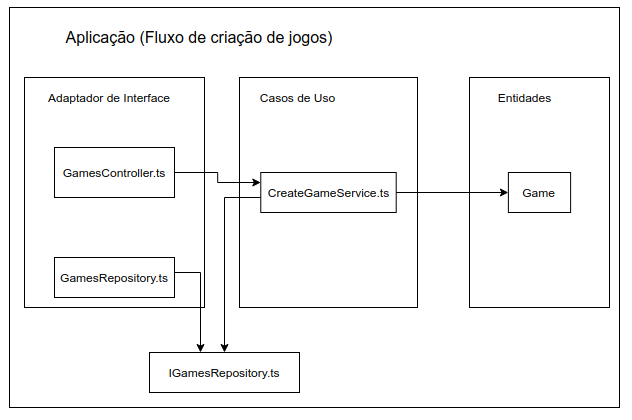
\includegraphics[scale=0.75]{Aplicacao_Limpa}
  \caption{Aplicação Limpa}
  \label{fig:insert_game}
\end{figure}

\end{subsecao}
\begin{subsecao}{Os benefícios}\label{subsec:dev_carch_benefits} 
  
\paragrafo{O benefício de adotar esse método de desenvolvimento se torna óbvio
ao necessitar reutilizar o caso de uso em algum outro fluxo da aplicação. Neste
caso, supondo que haja a necessidade de cadasterar grandes volumes de jogos na
nossa plataforma, seria mais conveniente passar toda essa informação através de
um arquivo do que inseri-la manualmente através de requisições Web. Por conta
disso, foi criado uma nova classe, GamesCreateBatch (Código \ref{alg:gamescreatebatch}), 
que processa um arquivo csv e invoca o serviço de criação de games para cada linha.}

\vspace{5mm}
\begin{lstlisting}[language=JavaScript, caption={Caso de Uso reaproveitado para processamento de arquivos},captionpos=b, label=alg:gamescreatebatch]
export default class GamesCreateBatch implements IBatchOperation {
  public async exec(): Promise<void> {
    //valida o nome do arquivo passado via linha de comando
    //cria lista de linhas

    const createGame = container.resolve(CreateGameService);

    await Promise.all(lines //percorre cada linha da lista criada
      .map(async (line: string): Promise<Game | boolean> => {
        try {
          //validacao da linha

          return await createGame.execute(/* conteudo da linha */));
        } catch (error) {
          return log.error(error);
        }
      }));
  }
}
\end{lstlisting}
\vspace{5mm}

\paragrafo{Como os níveis desse fluxo foram muito bem segregados ao longo dos
módulos, não foi necessário alterar nenhuma linha de código das classes
responsáveis por conhecer as regras de negócios da aplicação e das responsáveis
por interagir com o banco de dados.} 

\paragrafo{Outro ponto é que se em algum momento for necessário trocar o
\emph{Express JS}, somente a classe GamesController (Código \ref{alg:gamescontroller}) 
deverá sofrer uma manutenção, o restante, pelo menos referente a esse fluxo,
continuará intacto.} 

\paragrafo{Outro ganho da adoção desse método está na facilidade em testar os
componentes dessa aplicação. Para isso, foi criado a classe FakeGamesRepository
(Código \ref{alg:fakegamesrepository}), cujo propósito está em simular o acesso
ao banco de dados. Como essa classe é uma implementação da interface 
IGamesRepository, não haverá a necessidade de realizar nenhuma alteração no Caso
de Uso para se realizar dos testes ou, caso seja necessário, para trocar o 
\emph{TypeORM} por algum outro framework de acesso a banco de dados.}

\vspace{5mm}
\begin{lstlisting}[language=JavaScript, caption={Outra implementação do IGamesRepository},captionpos=b, label=alg:fakegamesrepository]
export default class FakeGamesRepository implements IGamesRepository {
  private games: Game[] = [];

  public async findByNameAndPublisherAndReleaseDate({
    name,
    publisher,
    release_date,
  }: ICreateGameDTO): Promise<Game | undefined> {
    return this.games.find(
      game => game.name === name && game.publisher === publisher,
    );
  }

  public async create(gameData: ICreateGameDTO): Promise<Game> {
    const game = new Game();
    Object.assign(game, { id: uuidv4() }, gameData);
    this.games.push(game);
    return game;
  }
\end{lstlisting}
\vspace{5mm}


\paragrafo{Com essa infraestrutura, o módulo CreateGameService.spec.ts (Código 
\ref{alg:creategametest}) testa, com simplicidade, 100\% das linhas do
Caso de Uso abordado.}

\vspace{5mm}
\begin{lstlisting}[language=JavaScript, caption={CreateGameService.spec.ts},captionpos=b, label=alg:creategametest]

import CreateGameService from '@modules/games/services/CreateGameService';
import AppError from '@shared/errors/AppError';
import FakeGamesRepository from '../fakes/repositories/FakeGamesRepository';

let fakeGamesRepository: FakeGamesRepository;
let createGame: CreateGameService;

describe('CreateGame', () => {
  beforeEach(() => {
    fakeGamesRepository = new FakeGamesRepository();
    createGame = new CreateGameService(fakeGamesRepository);
  });
  it('should be able to create a new game', async () => {
    const game = await createGame.execute({
      name: 'Cyberpunk',
      price: 80.0,
      publisher: 'CD Projekt Red',
      release_date: new Date(2021, 1, 1),
    });

    expect(game).toHaveProperty('id');
  });
  it('should not be able to create a duplicated game', async () => {
    const releaseDate = new Date(2021, 1, 1);
    await fakeGamesRepository.create({
      name: 'Cyberpunk',
      price: 80.0,
      publisher: 'CD Projekt Red',
      release_date: releaseDate,
    });
    await expect(
      createGame.execute({
        name: 'Cyberpunk',
        price: 80.0,
        publisher: 'CD Projekt Red',
        release_date: releaseDate,
      }),
    ).rejects.toBeInstanceOf(AppError);
  });
});
\end{lstlisting}
\vspace{5mm}

\end{subsecao}